
\section{Introduction}
% no \IEEEPARstart
% You must have at least 2 lines in the paragraph with the drop letter
% (should never be an issue)

With the vast involvement of streaming big data in many applications (e.g.,
stock market data, sensor data, social network data, etc.), quickly mining and
analyzing such data is becoming more and more important. 
% Many distributed stream processing frameworks such as Storm \cite{storm-web},
% Naiad \cite{Murray2013}, S4 \cite{Neumeyer2010}, TimeStream \cite{Qian2013},
% ELF \cite{Hu2014} have been developed to meet the requirements of big data
% real time processing. 
There is a recent trend in adapting batch-based data processing systems, such as
MapReduce \cite{Dean2004} and Spark \cite{Zaharia2010C}, to handle streaming
data by putting the input streams into micro-batches and treating the workloads
as a continuous series of small jobs.  Examples of such systems include HOP
\cite{Condie2010}, Comet \cite{He2010}, HStreaming \cite{HStreaming} and Spark
Streaming \cite{Zaharia2013}. 
Figure~\ref{fig:simplemodel} illustrates a simplified model of the data handling
pipeline in such systems. In this model, the \emph{batching module} receives and
divides the data streams into batches. Then, these batches are put into the
\emph{batch queue}. The \emph{processing module} schedules tasks for processing
according to the (BSP) model.  \begin{figure}[htbp] \centering
  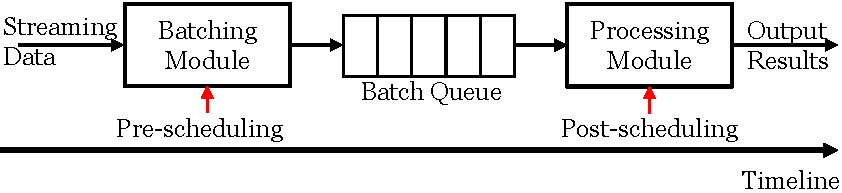
\includegraphics[width=0.40\textwidth]{FigureModel} \caption{A simplified
  model of the data processing pipeline in a batched stream processing
system.}\label{fig:simplemodel} \end{figure}

Batch stream processing systems become popular because not only they provide a
unified programming model to process batch data and streaming data, but also
they can leverage the fault tolerance and high throughput properties of the
batch processing frameworks~\cite{spark-summit}. However, in comparing to
record-at-a-time stream processing systems, such as Storm \cite{storm-web}, and
Naiad \cite{Murray2013}, batch steam processing systems often suffer from high
processing latency. Therefore, the fundamental challenge of building a batch
stream processing system is how to minimize the processing latency of each
micro-batch.
% The processing latency in such systems is mainly determined by the batch
% interval, therefore enabling the system to handle small batch intervals, such
% as milliseconds, is the key to address this question. 
This problem has recently attracted the community's interest, and some efforts, such
as \cite{drizzle}, have been focused on minimizing the coordination overhead of
processing the micro-batches, including the cost incured by task scheduling and
barriers between different processing stages. 
% , to surmount the limit on the batch intervals. 
In this paper, we focus on another issue, namely the straggler problem, where a
subset of workers straggling behind and significantly affecting the job
completion time. The straggler problem is a well-known critical problem in
parallel processing systems. As reported in
\cite{Ananthanarayanan2013} and \cite{Yadwadkar2014}, in the production clusters at
Facebook and Microsoft Bing, straggler tasks are on average 8 times slower than
the median task in the same job. 

% The average processing
% time of a micro-batch has to be smaller than the batch interval so that the
% system can keep up with the input load.  Hence, the existence of stragglers
% limits how small a batch interval can be set. 
% There exist efforts to solve the straggler problems in batch-based systems.
% However, they are not suitable for continuous processing of micro-batches. 
In comparing to processing of large batches, the straggler problems in
micro-batch processing are more severe and harder to tackle. First of all,
unlike processing large batches, where there are a large number of tasks to be
scheduled, the number of tasks in micro-batch processing is much more limited,
therefore, once a straggler occurs, we have little opportunity to mitigate the
problem by carefully scheduling the remaining tasks.  Second, batch processing
systems usually adopt the well-known bulk synchronous parallel (BSP) model,
where a barrier is placed at the end of each processing stage and all the
parallel tasks within the same stage have to synchronize at the barrier.  As a
batch stream processing system should handle many continuously recurring
micro-batches, if the execution times of the straggling tasks exceed the batch
interval, it would not only affect the latency of the current micro-batch, but
also the subsequent ones, which would suffer from unacceptable queueing latency.
Furthermore, the actions of handling stragglers have to be carried out very
quickly so that the total task (re-)scheduling and processing time should not
exceed the batch interval. This is especially challenging if we use small, say
sub-second, batch intervals. For example, the wait-speculate-re-execute paradigm
adopted in many existing solutions \cite{Dean2004} \cite{Zaharia2008}
\cite{Kwon2012} would be undesirable, because the processing time of the
micro-batches can be too short to afford the waiting time to detect the
stragglers, not to mention the additional latency incurred by relocating the
data and re-executing the straggling tasks. 

% Existing solutions assume one-time tasks over large data batch,
% instead of recurring micro-batches, therefore they are not suitable for batch
% stream processing systems. For example, we cannot adopt the
% wait-speculate-re-execute paradigm \cite{Dean2004} \cite{Zaharia2008}
% \cite{Kwon2012}, because the lifetime of the micro-batches can be too short to
% afford the waiting time to detect the stragglers.  Furthermore, most existing
% solutions (re-)schedule tasks after the batching module put the input data in
% the batch queue. We call these techniques as post-scheduling. These techniques
% would inherently incur high data movement cost, which is especially unaffordable
% for tasks handling micro-batches. 

We argue that the fundamental problem of using the existing straggler mitigation
solutions for micro-batch processing is that they detect (or predict)
stragglers and reschedule them too late in the data handling pipeline, i.e.
after the batching module has already dispatched the data into the batch queue
and the processing module has started processing the data
(recall Figure~\ref{fig:simplemodel}). The re-scheduling actions are carried out during
the task execution period, hence it would inevitably increase the processing
time of the micro-batches. Furthermore, as the data have already been
dispatched, re-scheduling would inherently incur expensive data relocation. Such
overhead would become significant in micro-batch processing due to the short
processing time of each micro-batch. We refer to this type of methods as
\emph{post-scheduling} techniques. To address the problem, we propose a new
\emph{pre-scheduling} framework, called \emph{Lever}, which predicts stragglers
and makes timely scheduling decisions to minimize the processing latency. Lever
utilizes the statistics of the processing of the previous batches to predict the
potential stragglers in the current batch and makes proactive re-scheduling
decisions to prevent stragglers. More specifically, Lever makes the
re-scheduling decisions before the batching module dispatches the data.
Therefore, the re-scheduling actions would not incur any data relocation, and, as
the scheduling is done while the data are being batched, it would not increase
the processing time of the micro-batch. 

We implemented Lever in Spark Streaming, which is contributed to the open source
community as an extension of Apache Spark. To the best of our knowledge, this is
the first work specifically addressing the straggler problem in continuous
micro-batch processing. In summary, this paper makes the following technical
contributions:

\begin{itemize}
  \item We discuss the behaviors of existing straggler mitigation methods and
	identify the problems of existing straggler mitigation methods for batch
	stream processing systems.

  \item To better mitigate stragglers when processing micro-batches, we present
	Lever, a pre-scheduling framework for handling straggler problems in batch
	stream processing systems. Lever predicts and re-schedules straggling tasks 
	before the dispatching the data and processing the tasks to avoid the
	latency incurred by the post-scheduling methods. Furthermore, by mitigating
	the stragglers, Lever can significantly reduce the processing latency of
	micro-batches.

  \item We propose various techniques to realize the new pre-scheduling
	framework. We propose a method to predict the potential stragglers before the
	execution of the tasks by using the historical statistics, which takes into
	account the variations of data streaming rates. In addition, we adopt the
	Iterative Learning Control model to estimate the capacity of the computing
	nodes. Finally, we propose two techniques to re-schedule the straggling
	tasks, which are suitable for a small and a large number of stragglers
	respectively. A method is proposed to automatically choose one out of these
	two techniques according the actual situation.

  \item We implemented Lever on Spark Streaming, and contributed it as
	an extension of Spark Streaming to the open source community.  Extensive
	experiments using both real and synthetic data show that Lever can mitigate
	stragglers efficiently and improve the performance of stream applications
	significantly.  

\end{itemize}

%   The rest of this paper is organized as follows. In Section II, we introduce the background and analyze the straggler problems in batched stream processing system. Section III describes the pre-scheduling strategy and the design of Lever. Section IV presents the implementation of Lever. We evaluate the performance of our system in Section V. Section VI briefly surveys the related works. Finally, Section VII concludes this paper.
